\documentclass{article}
\usepackage[margin=2.5cm]{geometry}
\usepackage{lipsum}
\usepackage{enumitem}

\usepackage{listings}
\lstdefinestyle{mystyle}{
    language=Matlab, % Cambia esto al lenguaje de programación deseado
    basicstyle=\ttfamily,
    frame=single,
    breaklines=true,
    showstringspaces=false,
}

\lstdefinestyle{mystyle2}{
    language=Python,
    basicstyle=\ttfamily,
    breaklines=true,
    showstringspaces=false,
}

\usepackage{graphicx}
\usepackage{setspace}
\usepackage{amsmath}
\onehalfspacing
\usepackage{authblk}
\renewcommand\Authfont{\normalsize}
\renewcommand\Affilfont{\itshape\small}
\usepackage{caption} % Se agregó el paquete caption

\title{\hrule height 5pt \\[2ex]\LARGE\bfseries Taller 1 - Imágenes Médicas\\ Conceptos Básicos: Matlab \& Python \\[2ex] \hrule height 1.3pt \\[2ex]\LARGE }
\renewcommand{\abstractname}{\Large \textbf{Resumen}}

\author{%
  \begin{minipage}[t]{0.25\textwidth}
    \centering
    \textbf{William Gómez Roa} \\ wa.gomez@javeriana.edu.co \\ Bioingeniería y Ciencia de Datos
  \end{minipage}%
  \begin{minipage}[t]{0.25\textwidth}
    \centering
    \textbf{Carolina Santos Baquero} \\ carolinasantosb@javeriana.edu.co \\ Bioingeniería
  \end{minipage}%
}

\date{}

\usepackage{changepage}

\begin{document}

\maketitle

\begin{adjustwidth}{1.4cm}{1.4cm}
\begin{abstract}
En este informe de Imágenes Médicas, se abordan conceptos básicos de procesamiento de imágenes utilizando Matlab y Python. Se exploran temas como la convolución de señales, análisis del contenido frecuencial de imágenes mediante la Transformada de Fourier, y la relación señal-ruido en el contexto de imágenes médicas. Además, se presenta una introducción al uso de la librería ITK en Python. Estos conceptos son fundamentales en el procesamiento y análisis de imágenes médicas, permitiendo mejorar la calidad de las imágenes y facilitar la detección de patrones y características relevantes para el diagnóstico médico.
\end{abstract}
\end{adjustwidth}



\section*{PARTE I: Conceptos básicos de imágenes en Matlab}

\subsection*{Ejercicio 1: Convolución de señales}
Modifique el código anterior para que la señal de entrada ya no sea una función tipo rampa, sino más bien una función tipo triángulo. Genere la gráfica de las señales donde se muestre el cambio de la función de entrada y de la respuesta al sistema usando esa nueva señal.

\begin{lstlisting}[style=mystyle]
% definir el tamaño del paso
dt = 0.1;

% definir la señal TRIÁNGULO f(t)
t1 = -2:dt:2;
Ft = -abs(t1) + 2;

% definir la segunda señal g(t).
t2 = -2:dt:2;
Gt = 3*ones(1, length(t2));

% generar la respuesta del sistema a la entrada con la convolución: Propiedad CONMUTATIVA f*g = g*f
yt = dt * conv(Ft, Gt);
yt_x = (1:length(yt)) * dt + t2(1) + t1(1);

%% graficar todas las señales

figure(1)
subplot(2, 2, 1)
plot(t1, Ft, 'r'), title('f(t) entrada del sistema')
grid on, xlim([-2 2])
xlabel('t'), ylabel('amplitud')

subplot(2, 2, 3)
plot(t2, Gt, 'b'), title('g(t)  respuesta al impulso')
grid on , ylim([0 3.5])
xlabel('t'), ylabel('amplitud')

subplot(2, 2, [2;4])
plot(yt_x, yt, 'k'), title('f(t)*g(t) respuesta del sistema')
grid on, xlabel('t'), ylabel('amplitud')

sgtitle('Convolución de Señales')
\end{lstlisting}


\begin{minipage}{\linewidth}
  \centering
  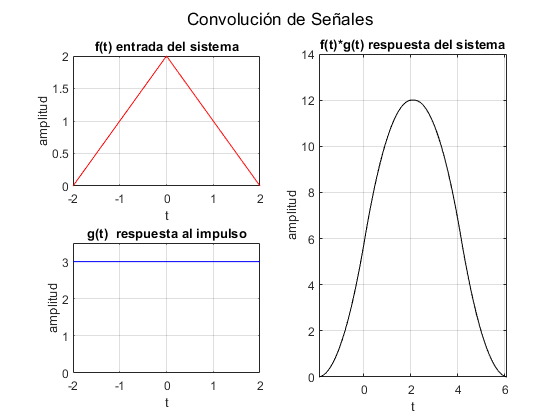
\includegraphics[width=0.7\textwidth]{imgs/p1.png}
  \captionof{figure}{Convolución $f(t)*g(t)$}
  \label{referenciarImagenAca}
\end{minipage}

\subsection*{Ejercicio 2: Convolución Suave}
Modifique el código anterior para agregar una nueva señal suave que genere un efecto intermedio entre la función rectangular y la función campana. Genere la gráfica de las señales donde se muestre la nueva señal agregada y la respuesta del sistema (simplificación) usando esa nueva señal. Es importante no eliminar las funciones rectangular y campana y sus resultados, para verificar el efecto de la nueva señal en comparación con las que ya se tenían.

\begin{lstlisting}[style=mystyle]
clc, clear, close all;

% definicion de la señal aleatoria
data = rand(1, 1000) - 0.5;

% definicion de las señales suaves
curv_rect = 1/61 * ones(1, 61);
t = 0:60;
curv_ham = -1/(61*2) * cos(1/61*2*pi*t) + 1/(61*2);

% Definicion de una señal INTERMEDIA
radio = 30;
circular = sqrt(radio^2 - (t-radio).^2);
circular = circular * (0.0164/30);

% aplicar la convolución sobre la señal aleatoria
rec_smooth = conv(data, curv_rect, 'same');
ham_smooth = conv(data, curv_ham, 'same');
cir_smooth = conv(data, circular, 'same');

% graficar todas las señales
figure(1)
subplot(2, 2, 1)
plot(data, 'k'), grid on, title('Señal aleatoria')
xlabel('x'), ylabel('y')

subplot(2, 2, 2)
plot(curv_rect, 'b', 'LineWidth', 2), title('Señales suaves'), grid on
hold on
plot(curv_ham, 'r', 'LineWidth', 2)
hold on
plot(circular, 'g', 'LineWidth', 2)
legend('Rectangular', 'Campana', 'Semi Círculo'), xlabel('x'), ylabel('y')

subplot(2, 2, [3, 4])
plot(rec_smooth, 'b', 'LineWidth', 2)
hold on
plot(ham_smooth, 'r', 'LineWidth', 2)
hold on
plot(cir_smooth, 'g', 'LineWidth', 2)
title('Señal simplificada por convolución'), grid on
\end{lstlisting}


\begin{minipage}{\linewidth}
  \centering
  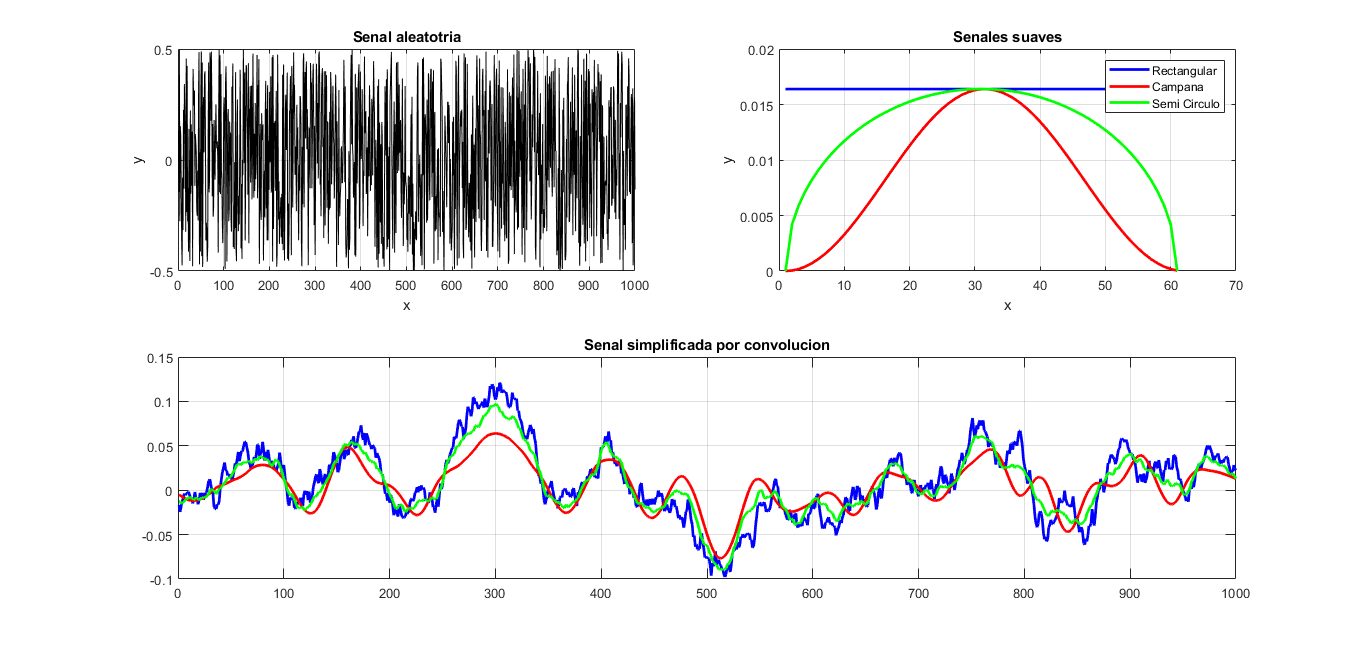
\includegraphics[width=1.0\textwidth]{imgs/p2.png}
  \captionof{figure}{Señal Intermedia}
  \label{referenciarImagenAca}
\end{minipage}


\subsection*{Ejercicio 3: Relación Señal Ruido}

¿Cuál será el efecto de variar la amplitud del ruido estimado para la señal? Genere otras dos estimaciones de ruido con amplitudes menores y mayores a la presentada en el ejemplo, y obtenga el valor de la relación señal a ruido para cada una de ellas. Analice qué pasa con los valores, y grafique también los diferentes ruidos estimados.

\begin{lstlisting}[style=mystyle]
clc, clear, close all;

% definicion de la longitud de las señales
length = linspace(-2*pi, 2*pi);

% definicion de la señal
signal1 = sin(length);

% definicion del ruido
noise1 = 0.5 * rand(size(signal1));
% definicion del ruido 2
noise2 = 0.1 * rand(size(signal1));
% definicion del ruido 3
noise3 = 1 * rand(size(signal1));

% calculo de la relacion señal a ruido
snr1 = snr(signal1, noise1);
% calculo de la relacion señal a ruido
snr2 = snr(signal1, noise2);
% calculo de la relacion señal a ruido
snr3 = snr(signal1, noise3);

% graficar la señal y el ruido estimado
figure(1)
subplot(2, 1, 1)
plot(signal1), title('Señal')
subplot(2, 1, 2)
plot(noise1)
hold on
plot(noise2)
hold on
plot(noise3), title('Ruidos')
legend('Ruido 1', 'Ruido 2', 'Ruido 3')
\end{lstlisting}

\begin{lstlisting}[style=mystyle]
snr1 =

    7.3210

snr2 =

   21.8749

snr3 =

    1.3105
\end{lstlisting}


\begin{minipage}{\linewidth}
  \centering
  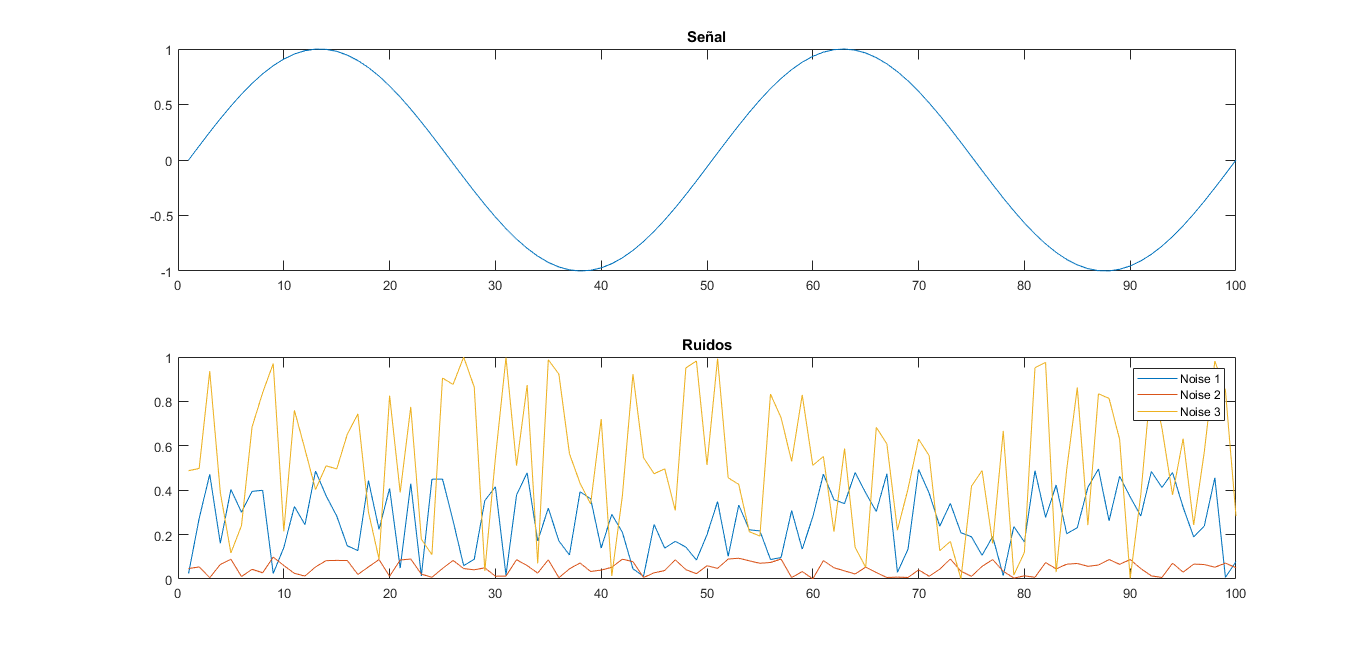
\includegraphics[width=1.0\textwidth]{imgs/p3.png}
  \captionof{figure}{Señal con distintas Amplitudes de Ruido}
  \label{referenciarImagenAca}
\end{minipage}

En este ejercicio, analizamos cómo la relación señal-ruido (SNR) afecta a una señal. La relación señal-ruido es una medida que nos indica cuánta energía de la señal es mayor que la energía del ruido presente en los datos. Una relación alta significa que la señal es fuerte en comparación con el ruido, mientras que una relación baja indica que el ruido domina la señal.

En resumen, al variar la amplitud del ruido estimado, podemos observar cómo la relación señal-ruido afecta la calidad de la señal y la interpretación de los datos.

\subsection*{Ejercicio 4: Transformada de Fourier}

¿Cuál será el efecto en el espectro de variar el contenido frecuencial de la imagen utilizada? Utilice el código ejemplo para visualizar el espectro de dos imágenes adicionales: una con poca información de bordes o detalles (una figura geométrica plana, por ejemplo) y otra con mucha información de altas frecuencias (una imagen con píxeles aleatorios, por ejemplo). Analice qué pasa con los espectros de las transformadas de Fourier de esas imágenes, incorporando los resultados obtenidos.

\begin{lstlisting}[style=mystyle]
clc, clear, close all

% cargar una imagen de ejemplo de MATLAB
imdata = imread('street2.jpg');
% obtener la versión en escala de grises de la imagen
g_imdata = rgb2gray(imdata);
% obtener la transformada de Fourier de la imagen
F = fft2(g_imdata);
% obtener el espectro centrado de frecuencias y orientaciones
Fsh = fftshift(F);
% aplicar una transformación logarítmica para facilitar la visualización
S2 = log(1 + abs(Fsh));
% finalmente, reconstruir la imagen original
F2 = ifftshift(Fsh);
f = ifft2(F2);


% visualizar las imágenes y el espectro de la transformada
figure(1)
subplot(2, 2, 1)
imshow(g_imdata), title('Imagen original (en escala de grises)')
subplot(2, 2, 3)
imshow(S2,[]), title('Espectro de la transformada de Fourier')
subplot(2, 2, 4)
imshow(f,[]), title('Imagen reconstruida')

%% 

% cargar una imagen de ejemplo de MATLAB
imdata_circle = imread('circulo.jpg');
% obtener la versión en escala de grises de la imagen
g_imdata_circle = rgb2gray(imdata_circle);
% obtener la transformada de Fourier de la imagen
F_circle = fft2(g_imdata_circle);
% obtener el espectro centrado de frecuencias y orientaciones
Fsh_circle = fftshift(F_circle);
% aplicar una transformación logarítmica para facilitar la visualización
S2_circle = log(1 + abs(Fsh_circle));
% finalmente, reconstruir la imagen original
F2_circle = ifftshift(Fsh_circle);
f_circle = ifft2(F2_circle);

% cargar una imagen de ejemplo de MATLAB
imdata_v = imread('voronoi.png');
% obtener la versión en escala de grises de la imagen
g_imdata_v = rgb2gray(imdata_v);
% obtener la transformada de Fourier de la imagen
F_v = fft2(g_imdata_v);
// obtener el espectro centrado de frecuencias y orientaciones
Fsh_v = fftshift(F_v);
// aplicar una transformación logarítmica para facilitar la visualización
S2_v = log(1 + abs(Fsh_v));
// finalmente, reconstruir la imagen original
F2_v = ifftshift(Fsh_v);
f_v = ifft2(F2_v);

// visualizar las imágenes y el espectro de la transformada
figure(2)
subplot(2, 2, 1)
imshow(g_imdata_circle), title('Imagen original CIRCULO (en escala de grises)')
subplot(2, 2, 3)
imshow(S2_circle,[]), title('Espectro de la transformada de Fourier CIRCULO')
subplot(2, 2, 4)
imshow(f_circle,[]), title('Imagen reconstruida CIRCULO')
sgtitle('Imagen de Baja Frecuencia')


figure(3)
subplot(2, 2, 1)
imshow(g_imdata_v), title('Imagen original VORONOI (en escala de grises)')
subplot(2, 2, 3)
imshow(S2_v,[]), title('Espectro de la transformada de Fourier VORONOI')
subplot(2, 2, 4)
imshow(f_v,[]), title('Imagen reconstruida VORONOI')
sgtitle('Imagen de Alta Frecuencia')

\end{lstlisting}


\begin{minipage}{\linewidth}
  \centering
  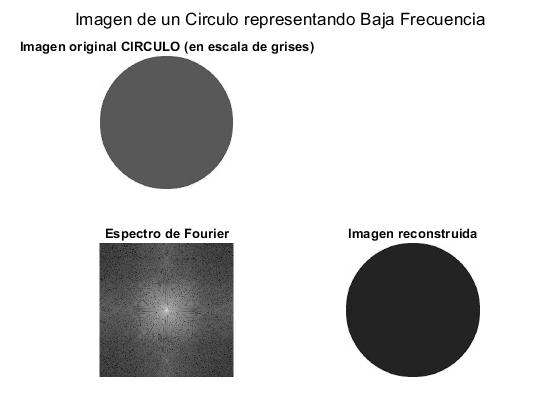
\includegraphics[width=0.7\textwidth]{imgs/p4_1.png}
  \captionof{figure}{Imágen de Baja Frecuencia}
  \label{referenciarImagenAca}
\end{minipage}


\begin{minipage}{\linewidth}
  \centering
  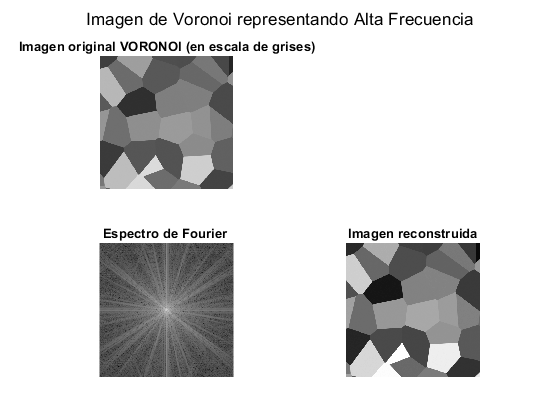
\includegraphics[width=0.7\textwidth]{imgs/p4_2.png}
  \captionof{figure}{Imágen de Alta Frecuencia}
  \label{referenciarImagenAca}
\end{minipage}

En este ejercicio, utilizamos la transformada de Fourier para analizar el espectro de dos imágenes adicionales: una imagen de un círculo y una imagen de voronoi. Para ello, primero aplicamos la transformada de Fourier a cada imagen para obtener el espectro de frecuencias. En la imagen del círculo, que tiene un contenido frecuencial bajo al ser una figura geométrica plana, el espectro mostró una distribución concentrada en bajas frecuencias. Por otro lado, en la imagen de voronoi, que contiene muchos detalles y bordes, el contenido frecuencial fue alto, lo que resultó en un espectro más disperso y con mayor presencia de altas frecuencias.

En respuesta a la pregunta sobre el efecto de variar el contenido frecuencial de las imágenes en el espectro, podemos concluir que imágenes con contenido frecuencial bajo mostrarán un espectro más concentrado en bajas frecuencias, mientras que imágenes con contenido frecuencial alto tendrán un espectro más disperso con una mayor presencia de altas frecuencias. En otras palabras, imágenes con detalles finos y bordes definidos tendrán un espectro con una mayor distribución en frecuencias más altas, mientras que imágenes más uniformes o suaves mostrarán un espectro más centrado en bajas frecuencias. La transformada de Fourier nos permite entender cómo se distribuyen las frecuencias en una imagen y permite el análisis y procesamiento de imágenes en el dominio de la frecuencia.

\section*{PARTE II: Instalación y uso básico de librería ITK en Python}

\subsection*{Ejercicio 5: Uso de la librería \textit{itk}}

Utilice el código del segundo ejemplo para generar versiones en escala de grises de 3 imágenes, con diferentes contenidos de color. Incluya en el informe el código utilizado para cada imagen, así como las imágenes de entrada y salida en cada caso.

\begin{lstlisting}[style=mystyle2]
import itk

# definir la imagen de entrada con 3 canales (color) y dos dimensiones
InputImageType = itk.Image[itk.RGBPixel[itk.UC], 2]
# definir la imagen de salida con 1 canal (gris) y dos dimensiones
OutputImageType = itk.Image[itk.UC, 2]

# definir un lector para la imagen de entrada e inicializarlo
reader = itk.ImageFileReader[InputImageType].New()

# definir un proceso para cambiar los canales de la imagen (color a gris)
rgbFilter = itk.RGBToLuminanceImageFilter.New()

# definir un escritor para la imagen de salida e inicializarlo
writer = itk.ImageFileWriter[OutputImageType].New()

# asignar al lector el nombre del archivo de entrada
reader.SetFileName("fundus.jpg")
# asignar al escritor el nombre del archivo de salida
writer.SetFileName("g_fundus.jpg")
# conectar el proceso al lector para tomar la imagen de entrada
rgbFilter.SetInput(reader.GetOutput())
# conectar el escritor al proceso para tomar la imagen de salida
writer.SetInput(rgbFilter.GetOutput())
# ejecutar la linea de procesamiento completa
writer.Update()

\end{lstlisting}
\begin{minipage}{\linewidth}
  \centering
  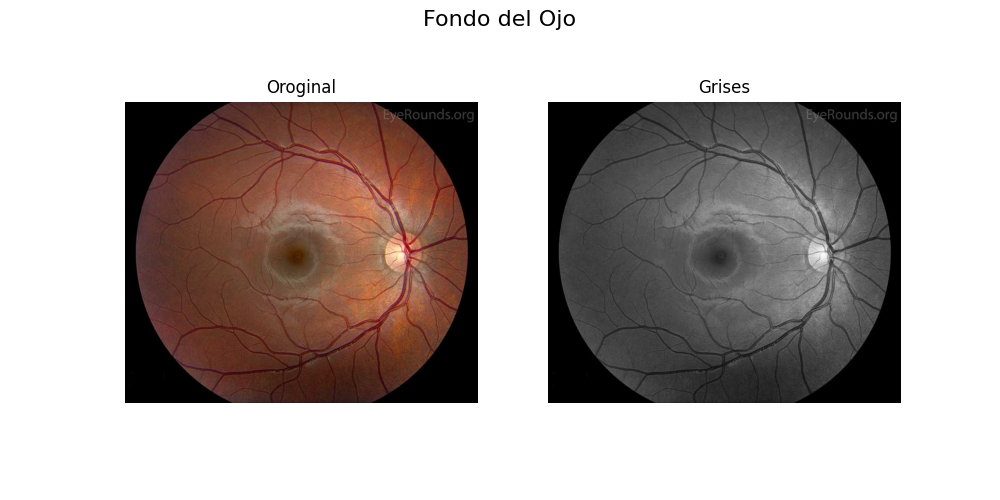
\includegraphics[width=0.7\textwidth]{imgs/fundus.png}
  \captionof{figure}{Imaágen del Fondo del Ojo de alta definición.}
  \label{referenciarImagenAca}
\end{minipage}


\begin{lstlisting}[style=mystyle2]
import itk

# definir la imagen de entrada con 3 canales (color) y dos dimensiones
InputImageType = itk.Image[itk.RGBPixel[itk.UC], 2]
# definir la imagen de salida con 1 canal (gris) y dos dimensiones
OutputImageType = itk.Image[itk.UC, 2]

# definir un lector para la imagen de entrada e inicializarlo
reader = itk.ImageFileReader[InputImageType].New()

# definir un proceso para cambiar los canales de la imagen (color a gris)
rgbFilter = itk.RGBToLuminanceImageFilter.New()

# definir un escritor para la imagen de salida e inicializarlo
writer = itk.ImageFileWriter[OutputImageType].New()

# asignar al lector el nombre del archivo de entrada
reader.SetFileName("oct.jpg")
# asignar al escritor el nombre del archivo de salida
writer.SetFileName("g_oct.jpg")
# conectar el proceso al lector para tomar la imagen de entrada
rgbFilter.SetInput(reader.GetOutput())
# conectar el escritor al proceso para tomar la imagen de salida
writer.SetInput(rgbFilter.GetOutput())
# ejecutar la linea de procesamiento completa
writer.Update()

\end{lstlisting}
\begin{minipage}{\linewidth}
  \centering
  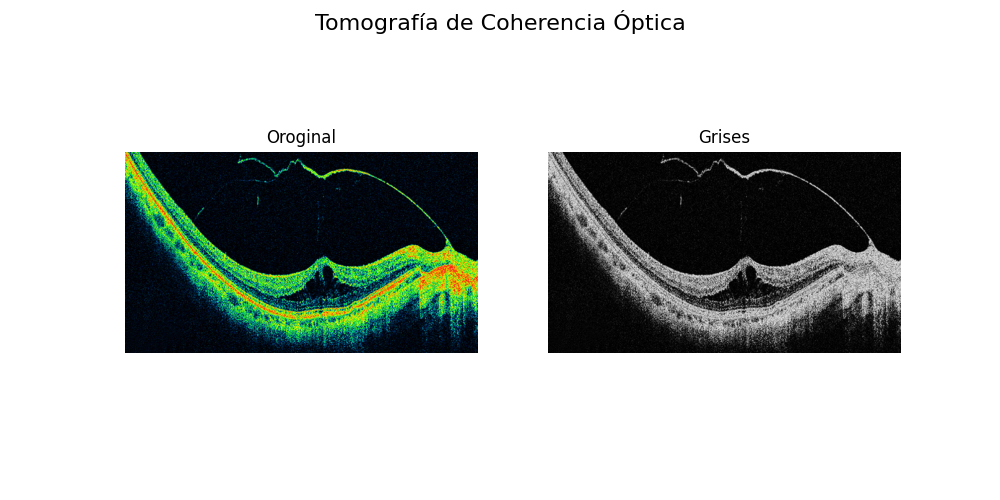
\includegraphics[width=0.7\textwidth]{imgs/oct.png}
  \captionof{figure}{Tomografía de Coherencia Óptica.}
  \label{referenciarImagenAca}
\end{minipage}


\begin{lstlisting}[style=mystyle2]
import itk

# definir la imagen de entrada con 3 canales (color) y dos dimensiones
InputImageType = itk.Image[itk.RGBPixel[itk.UC], 2]
# definir la imagen de salida con 1 canal (gris) y dos dimensiones
OutputImageType = itk.Image[itk.UC, 2]

# definir un lector para la imagen de entrada e inicializarlo
reader = itk.ImageFileReader[InputImageType].New()

# definir un proceso para cambiar los canales de la imagen (color a gris)
rgbFilter = itk.RGBToLuminanceImageFilter.New()

# definir un escritor para la imagen de salida e inicializarlo
writer = itk.ImageFileWriter[OutputImageType].New()

# asignar al lector el nombre del archivo de entrada
reader.SetFileName("hand.jpg")
# asignar al escritor el nombre del archivo de salida
writer.SetFileName("g_hand.jpg")
# conectar el proceso al lector para tomar la imagen de entrada
rgbFilter.SetInput(reader.GetOutput())
# conectar el escritor al proceso para tomar la imagen de salida
writer.SetInput(rgbFilter.GetOutput())
# ejecutar la linea de procesamiento completa
writer.Update()

\end{lstlisting}
\begin{minipage}{\linewidth}
  \centering
  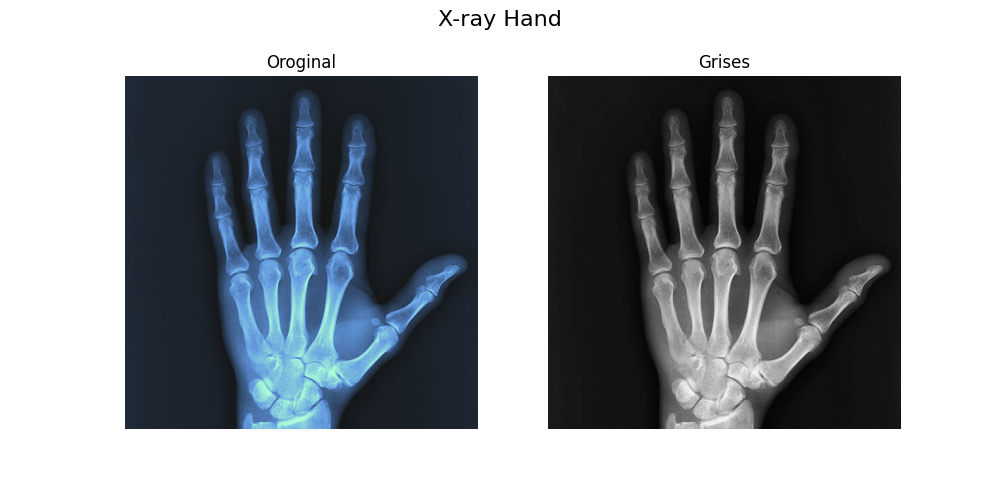
\includegraphics[width=0.7\textwidth]{imgs/hand.png}
  \captionof{figure}{Rayos X}
  \label{referenciarImagenAca}
\end{minipage}


En este ejercicio, utilizamos la librería \textit{itk} para generar versiones en escala de grises de tres imágenes con diferentes contenidos de color. 

Para cada imagen, leemos la imagen de entrada con el lector, luego aplicamos el proceso de conversión de color a gris con el filtro \textit{RGBToLuminanceImageFilter}, y finalmente escribimos la imagen resultante en escala de grises en un archivo de salida.

\end{document}